%Przykładowy plik ułatwiający złożenie projektu dyplomowego inżynierskiego.
%UWAGA: Generowany napis na stronie tytułowej o treści PROJEKT DYPLOMOWY INŻYNIERSKI został zaproponowany przeze mnie i nie jest, póki co, potwierdzony przez władze wydziału. Przed ostatecznym oddaniem tak złożonej pracy należy upewnić się jaka powinna być treść tego napisu. W momencie gdy uzyskam informację na temat treści tego napisu, dokonam niezbędnych zmian w źródłach.

\documentclass[eng,printmode]{mgr}
%opcje klasy dokumentu mgr.cls zostały opisane w dołączonej instrukcji

%poniżej deklaracje użycia pakietów, usunąć to co jest niepotrzebne
\usepackage{polski} %przydatne podczas składania dokumentów w j. polskim
%\usepackage[polish]{babel}%alternatywnie do pakietu polski, wybrać jeden z nich
\usepackage[utf8]{inputenc} %kodowanie znakĂłw, zaleĹĽne od systemu
\usepackage[T1]{fontenc} %poprawne składanie polskich czcionek

%pakiety do grafiki
\usepackage{graphicx}
%\usepackage{subfigure}
\usepackage{psfrag}

%pakiety dodające dużo dodatkowych poleceń matematycznych
\usepackage{amsmath}
\usepackage{amsfonts}

%pakiety wspomagające i poprawiające składanie tabel
%\usepackage{supertabular}
\usepackage{array}
\usepackage{tabularx}
\usepackage{hhline}

%pakiet wypisujący na marginesie etykiety równań i rysunków zdefiniowanych przez \label{}, chcąc wygenerować finalną wersję dokumentu wystarczy usunąć poniższą linię
%\usepackage{showlabels}

%definicje własnych poleceń
\newcommand{\R}{I\!\!R} %symbol liczb rzeczywistych, działa tylko w trybie matematycznym
\newtheorem{theorem}{Twierdzenie}[section] %nowe otoczenie do składania twierdzeń

%dane do złożenia strony tytułowej
\title{Detekcja aktywności mówcy w systemach automatycznego rozpoznawania mowy}
\engtitle{Voice activity detection in automatic speech recognition systems}
\author{Paulina Szczerbak}
\supervisor{Prof. dr hab. inż. Ryszard Makowski}
%\guardian{dr hab. inż. Imię Nazwisko Prof. PWr, I-6} %nie używać jeśli opiekun jest tą samą osobą co prowadzący pracę

%\date{2008} %standardowo u dołu strony tytułowej umieszczany jest bieżący rok, to polecenie pozwala wstawić dowolny rok

%poniżej jest lista kierunków i specjalności na wydziale elektroniki, należy wybrać właściwe lub dopisać jeśli nie ma odpowiednich
\field{Automatyka i Robotyka (AIR)}
\specialisation{Technologie informacyjne w systemach automatyki (ART)}

%tutaj zaczyna się właściwa treść dokumentu
\begin{document}
\bibliographystyle{plabbrv} %tylko gdy uĹĽywamy BibTeXa, ustawia polski styl bibliografii

\maketitle %polecenie generujące stronę tytułową
%\dedication{6cm}{Dla mamy i taty heheheheheh xD \texttt{$\backslash$dedykacja}}

\tableofcontents %spis treści

%poniżej znajduje się przykładowa treść dalszej części dokumentu, zainteresowanych zachęcam do rozszyfrowania frazy "Lorem ipsum" :)
\chapter{Wstęp}
Celem niniejszej pracy jest zaprezentowanie wybranych metod detekcji aktywności mówcy (VAD) w systemach automatycznego rozpoznawania mowy w oparciu o napisany program w języku C++. Kolejnym etapem jest porównanie zaimplementowanych metod pod względem dokładności detekcji w separowanych wyrazach oraz w dłuższych ciągach słów.

Rozdział 2. opisuje w uproszczony sposób proces wytwarzania mowy przez człowieka. Prezentuje, w jaki sposób działa aparat mowy oraz z jakich narządów się składa. Wyjaśnione zostaje zagadnienie fonemów oraz ich wykorzystanie w polskim alfabecie. Na koniec pokazany jest matematyczny model jaki można stworzyć wzorując się na naturalnym systemie generowania mowy.

Rozdział 3. zawiera wyjaśnienie na temat detekcji aktywności mówcy - czym jest oraz gdzie jest wykorzystywana. W tym rodziale opisane są również wybrane algorytmy, które zostały zestawione w dalszej części pracy. Przedstawiona jest zasada ich działania oraz pokrótce wyjaśniona kwestia implementacyjna każdego z nich.
 
Rozdział 4. prezentuje wyniki działania wybranych algorytmów dla separowanych słów. Pokazane są różnice w detekcji oraz ocena każdego z algorytmów.

Rozdział 5. zawiera  wyniki detekcji dla całych ciągów słów oraz porównanie w działaniu wybranych algorytmów i ich ocenę.

\chapter{Generowanie sygnału mowy}
 \section{Mowa w życiu człowieka}
 
 Mowa w życiu większości ludzi stanowi podstawę komunikacji interpersonalnej. Jest sygnałem akustycznym, czyli rozważany jest zakres częstotliwości słyszanych przez człowieka, to jest od 20Hz do 16kHz. Zatem mowa to nic innego jak system artykułowanych dźwięków, które układają się zgodnie z konwencją wybranego języka. Pełni ona funkcję nie tylko komunikacyjną (przekazywanie informacji drugiej osobie o tym, co doświadczyliśmy, czy czego się dowiedzieliśmy), ale również ekspresyjną (można w niej zawrzeć informacje o emocjach nadawcy) oraz regulacyjną (wydawanie i przyjmowanie dyspozycji). 
 
 
 \section{Biologiczny proces generowania mowy}
 Wszelkie metody przetwarzania sygnału mowy muszą bazować na strukturze sygnału, a ta jest niewątpliwie uzależniona od sposobu, w jaki jest on wytwarzany. Niegdyś generowanie sygnałów mowy było domeną jedynie organizmu człowieka, czyli systemu naturalnego. W celu stworzenia systemu, który w jakiś sposób operuje na sygnałach mowy, czyli np. syntezatora mowy, systemu generującego sygnały mowopodobne, systemu automatycznego rozpoznawania mowy czy detekcji aktywności mówcy, należy mieć przynajmniej podstawową wiedzę na temat systemu naturalnego - tego, w jaki sposób działa aparat mowy człowieka.
 
 Wytwarzanie mowy przez człowieka jest procesem niezwykle skomplikowanym, który ma swój początek w mózgu, gdzie następuje konstrukcja wypowiedzi. Później następuje sformułowanie fonetyki i artykulacja poprzez aparat mowy. Ponadto, w procesie generowania mowy można wyróżnić cztery pomniejsze etapy:
	 
	 - proces psychologiczny - wymyślenie i skonstruowanie wypowiedzi,
	 
	 - proces neurologiczny - pobudzenie przez układ nerwowy mięśni, które biorą udział w wytwarzaniu mowy,
	 
	 - proces fizjologiczny - proces kształtowania dźwięków mowy ludzkiej,
	 
	 - proces aerodynamiczny - drgania i przepływ powietrza przez aparat mowy. 
  
  Pierwszym narządem wchodzącym w skład traktu głosowego człowieka są płuca - dostarczają one powietrze do procesu artykulacji, są źródłem zmian ciśnienia akustycznego. Organ mowy człowieka jest napędzany przez wydychane powietrze. Powietrze to, jest prowadzone przez oskrzela i tchawicę do krtani, a drgające w niej struny głosowe modyfikują ciśnienie i wytwarzają dźwięczne fragmenty mowy.  Następnie, dzięki wnękom rezonansowym, tworzonym przez język, podniebienie, zęby oraz wargi, dźwięk ten jest modulowany. Niezwykle ważną rolę przy formowaniu tych wnęk, odgrywają ruchy żuchwy i policzków. Podczas generowania głosek nosowych zamknięta jama ustna spełnia rolę bocznika akustycznego, a dzięki odpowiedniemu ustawieniu języczka podniebienia miękkiego, fala dźwiękowa jest emitowana przez jamę nosową i nozdrza. Struktura traktu głosowego jest przedstawiona schematycznie na rysunku 2.1.

\begin{figure}
	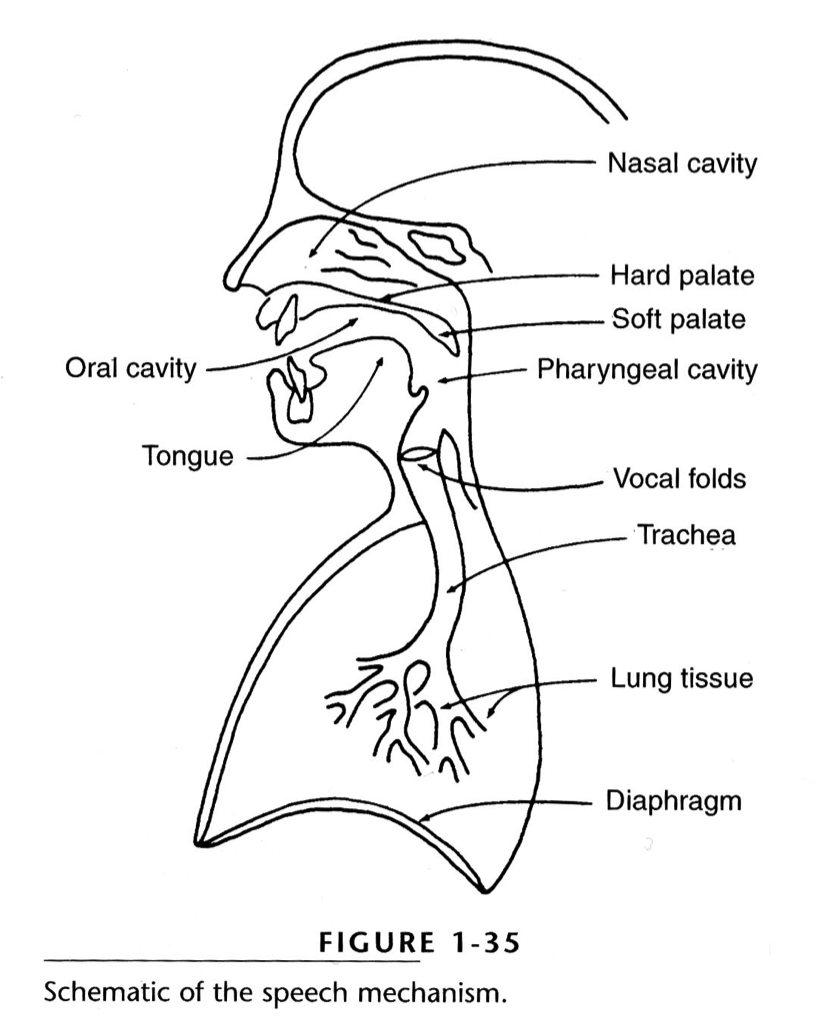
\includegraphics[scale=0.45]{speechmech.png}
	\caption{Aparat mowy człowieka}
\end{figure}

 Ponadto, sterowanie całym systemem generowania mowy jest bardzo złożone i w dużej mierze opiera się na licznych sprzężeniach zwrotnych. Główną rolę odgrywa tutaj sprzężenie zwrotne, które poddaje jakość wydawanych dźwięków bezpośredniej ocenie poprzez analizator słuchowy. Dzięki temu proces artykulacji jest odpowiednio sterowany. Istotę tego sprzężenia zwrotnego potwierdzają trudności z mową wśród ludzi głuchych oraz ludzi słyszących, którzy tymczasowo przebywają w trudnych warunkach środowiskowych, które uniemożliwiają słyszenie własnego głosu.
 
 SCHEMAT Z PDFA STR 23 SPRZERZENIE ZWROTNE  
  
 \section{Jednostki fonetyczne}
 W celu przeprowadzania badań nad sygnałem mowy, należy wprowadzić jednostkę, która ułatwi wykonywanie operacji na całych słowach. Należy tutaj zaznaczyć, że słowo to dźwiękowy odpowiednik wyrazu, a wyraz to zapis słowa. Każde słowo zawiera w sobie przynajmniej jedną sylabę, każdą sylabę można również podzielić na mniejsze stany. W związku z tym, że każdy wyraz zawiera w sobie ciąg liter, to najczęściej wyróżnianymi elementami słowa są fonemy, zwane również głoskami. W większości przypadków na każdy fonem przypada odpowiadająca mu litera, ale są fonemy, które takiego odpowiednika nie posiadają. Istotne jest rownież, że każda litera może mieć różną reprezentację akustyczną w zależnośći od sąsiadujących z nią fonemów. Listę fonemów języka polskiego przedstawiono w tabeli 2.3.1.
 
 TABELA Z FONEMAMI MOWY POLSKIEJ
 
 \section{Matematyczny model procesu generowania mowy}
 
 

\chapter{Wybrane metody detekcji aktywności mówcy}
 \section{Czym jest detekcja aktywności mówcy oraz gdzie się ją wykorzystuje}
 + schemat jak w ksiazce RM, w ktorym miejscu jest vad w systemie ARM
 
 Detekcja aktywności mówcy (Voice Activity Detection - VAD) jest powszechnie stosowana w systemach automatycznego rozpoznawania mowy. Podczas rejestrowania wypowiedzi do późniejszego przetwarzania jej przez system ARM, zostaje zarejestrowana cała wypowiedź mówcy, włącznie z częścią, która nie zawiera mowy. Jeżeli we fragmencie jest zawarty sygnał mowy, mówimy, że mówca jest aktywny. Aktywnością mówcy nazywa się emitowny przez niego dźwięk.  Zawartość semantyczna wypowiedzi jest zawarta w głównej mierze we fragmentach, kiedy mówca jest aktywny. Analizowanie całego  zarejestrowanego sygnału mowy, bez wykorzystania systemu VAD, jest oczywiście możliwe, aczkolwiek niepotrzebnie zwiększa czas obliczeń oraz istnieje prawdopodobieństwo, że fragment, gdy mówca nie jest aktywny, zostanie błędnie zaklasyfikowany jako jakiś konkretny fonem - zatem w dużej mierze może popsuć jakość rozpoznania. Detekcja aktywności mówcy w ogólnym przypadku zakłada, że sygnał może występować w dwóch stanach: tylko szum (brak sygnału mowy), szum + sygnał mowy. Korzystając z zagadnienia hipotez ze statystyki, możemy pierwszy stan oznaczyć jako hipotezę $H_{0}$, a drugi jako $H_{1}$, dzięki czemu możemy przedstawić to w następujący sposób:
 \begin{equation}
  \begin{array}{c}
	  H_{0}: f(n)=x(n)\\
	  H_{1}: f(n)=v(n)+x(n)
  \end{array} 	 
 \end{equation}
  Przy takim rozumowaniu konieczne jest określenie statystyki $S(n)$ sygnału, dzięki czemu możliwe będzie dokonywanie detekcji, a w dalszej kolejności zastosowanie kryterium decyzyjnego. Kryterium decyzyjne zwykle polega na porównaniu wartości $S(n)$ z progiem detekcji, który w mniej skomplikowanych algorytmach przyjmuje stałą wartość. Natomiast w tych bardziej złożonych, może występować np. jako funkcja czasu. Wartość stałej wartości progu jest ustalana w wyniku teoretycznych rozważań lub empirycznie. Zatem detekcja $\gamma(n)$, w ogólnej postaci, będzie prezentować się następująco:
   \begin{equation}
   \begin{array}{c}
	   S(n)\geq\gamma(n)\to H_{1}\\
	   S(n)<\gamma(n)\to H_{0}
   \end{array} 	 
   \end{equation}
 
	MIARY JAKOSCI DETEKCJI DODATEK D 
 

 \section{Algorytm bazujący na energii pojedynczej ramki}
 \section{Algorytm bazujący na obwiedni sygnału}
 \section{Algorytm SFF (Single Frequency Filtering)}
 tłumaczenie artykułu:
 
 Podstawowe informacje w podejściu Single Frequency Filtering
 
 Sygnał mowy ma zależności zarówno z czasem, jak i z częstotliwością. Skutkuje to tym, że SNR (Signal to Noise Ratio) jest funkcją w dziedzinie czasu oraz w dziedzinie częstotliwości. Dla idealnego szumu o danej całkowitej mocy, moc jest podzielona równo dla każdej częstotliwości, podczas gdy dla sygnału moc jest rozdzielona nierównomiernie dla częstotliwości. Zatem, $S^2(f)/N^2(f)$ jest wyższe dla niektórych częstotliwości i niższe dla innych, gdzie S(f) i N(f) są amplitudami sygnału i szumu jako funkcja w dziedzinie częstotliwości. To daje dużo wyższe wartości dla średniej wartości  $S^2(f)/N^2(f)$ powyżej zakresu częstotliwości w porównaniu ze stosunkiem całkowitej mocy sygnału do całkowitej mocy szumu powyżej całkowitego zakresu częstotliwości. 
 
 Przyjmijmy wzory (1), (2), (3) z artykułu, gdzie (fi - fi+1)
 jest (i+1)-tą przerwą spośród L nienachodzących na siebie pasm częstotliwościowych oraz i=0,1,...,L-1. Obowiązuje następująca nierówność:
 
 alfa >= beta >= gamma (4)
 
 S(f) i N(f) są obliczane dla zdegradowanego wyrażenia mowy i dla szumu używając 512-punktowej DFT dla segmentów zokienkowanych oknem Hanna o rozmiarze 20msec dla KAŻDEGO PRZESUNIĘCIA PRÓBKI używając L=16. W Tabeli I (artykuł) przedstawiono średnie wartości alfa, beta, gamma obliczone dla całego wyrażenia. Oczywiste jest, że średine alfa >= średnie beta >= średnie gamma dla różnych typów szumu. W przypadku dla szumu białego wartości sr alfa, sr beta, sr gamma są niższe niż wartości dla niestacjonarnych szumów(np volvo i karabin maszynowy). W przypadku dla szumów niestacjonarnych dolna granica jest niska dla niektórych częstotliwości, co sprawia, że mianownik N(f) jest mały. Z małymi wartościami w mianowniku, współczynniki alfa, beta gamma są relatywnie wyższe, jak zaobserwowano w Tabeli I w srednich wartosciach alfa, beat, gamma dla szumu volvo i karabinu maszynowego. Warto również zauważyć, że dla szumów rozłożonych nierównomiernie, taich jak karabin maszynowy, f16 i volvo, wartości sr alfa i sr beta są dużo wyższe niż dla większości szumów rozłożonych równomiernie, taich jak szum biały, różowy i buccaneer2, podczas gdy odpowiadające im wartości sr gamma są niskie we wszystkich przypadkach. Ma to związek z obszarami zawierającymi wysoki S(f)/N(f) (SNR) w dziedzinie czasu i dziedzinie częstotliwości dla szumów rozłożonych nierównomiernie.
 
 Moc sygnału i szumu jako funkcja w dziedzinie częstotliwości może zostać obliczona wykorzystując  blokowe przetwarzanie jak w DFT lub poprzez filtrowanie przez SFF, jak opisano w następnej skcji. Tabela II pokazuje, że nierówność (4) obowiązuje również w podejściu SFF. Oczekuje się, że zarówno podeście oparte o DFT, jak i SFF dadzą podobne rezultaty. Podejście SFF zostało tutaj wykorzystane, ponieważ dzięki niemu mozna uniknąć niektórych skutków spowodowanych blokowym przetwarzaniem. Również obliczenia dla SFF są szybsze w porównaniu z obliczeniami w DFT w każdej chwili próbkowania.
 
 
 Proponowany algorytm VAD 
 
 A. Obwiednia sygnału mowy w każdej częstotliwości
 
 Sygnał mowy w zdyskretyzowanej dziedzinie czasu s(n) jest różnicowany i zróżnicowany sygnał jest rozumiany jako x(n) = s(n) -s(n-1). Częstotliwość próbkowania to fs. Sygnał x(n) jest przemnażany przez zespolona sinusoidę o danej znormalizowanej częstotliwości śr omega k. Wynikowa operacja w dziedzinie czasu jest dana jako: 
 
 $xk(n) = x(n)e^(j śromegak n)$, gdzie 
 
 $śr omega k = (2pi*śr_fk)/fs.$
 
 Kiedy pomnożymy x(n) przez $e^(j*śr_omega_k*n)$, wynikowe widmo xk(n) będzie przesuniętym widmem x(n). Czyli,
 
$ Xk(omega) = X(omega - śr_omega_k)$,
 gdzie Xk(omega) i X(omega) to odpowiednio widma xk(n) i x(n).
 
 Sygnał xk(n) jest przepuszczany przez jednobiegunowy filtr, którego transmitancja jest dana jako:
 
 $H(z) = 1/(1+rz^(-1)).$
 
 Jednobiegunowy filtr ma biegun na osi liczb rzeczywistych w odległości r od początku układu współrzędnych. Lokalizacja pierwiastka jest w z = -r na płaszczyśnie liczb zespolonych , co odpowiada połowie częstotliwości próbkowania, np fs/2. Wyjście filtra yk(n) jest dane jako:
 
 yk(n) = -r *yk(n-1)+xk(n)
 
 Obwiednia sygnału yk(n) jest dana jako:
 
 $ek(n) = sqrt(ykr^2(n) + yki^2(n))$ (10) , 
 
   gdzie ykr(n) i yki(n) są odpowiednio częścią rzeczywista i urojoną yk(n).
 
 Kiedy filtrowanie xk(n) będzie zrobione dla fs/2, powyższa obwiednia ek(n) będzie odpowiadać obwiedni sygnału xk(n) przefiltrowanego w pożądanej częstotliwości 
 
 $fk = fs/2 - śr_fk.$
 
 
 Powyższa metoda estymowania obwiedni składowej dla częstotliwości fk jest określana jako podejście single frequency filtering (SFF). 
 

\chapter{Implementacja programu}

\chapter{Wyniki dla pojedynczych słów}
 \section{Sposób oceny}
Donec cursus nulla vitae pede. Etiam quam pede, aliquet ut, pellentesque sed, sagittis non, est. Quisque egestas malesuada risus. Maecenas ultricies libero a quam. Nullam feugiat arcu. Class aptent taciti sociosqu ad litora torquent per conubia nostra, per inceptos hymenaeos. In interdum, risus ut gravida sollicitudin, leo sapien commodo dui, non consectetuer nisl nunc ac massa. Mauris a orci in eros venenatis euismod. Curabitur orci. Quisque pharetra, dui sed dignissim hendrerit, nibh ante malesuada eros, sed tincidunt magna lorem a tellus. Aliquam erat volutpat. Aenean pulvinar, metus et mattis dictum, massa lacus semper purus, quis vehicula augue mi et leo. Ut eu ipsum. Sed dictum dapibus nisi. Cras mattis. Nulla sed augue ac sem tempus condimentum. 
 \section{Wyniki}

\chapter{Wyniki dla ciągów słów}

\chapter{Podsumowanie}

\addcontentsline{toc}{chapter}{Bibliografia} %utworzenie w spisie treści pozycji Bibliografia
\bibliography{bibliografia} % wstawia bibliografię korzystając z pliku bibliografia.bib - dotyczy BibTeXa, jeżeli nie korzystamy z BibTeXa należy użyć otoczenia thebibliography
%biologiczny proces
%http://otworzksiazke.pl/images/ksiazki/sygnal_mowy/sygnal_mowy.pdf
%
%http://www.iaeng.org/IJCS/issues_v36/issue_4/IJCS_36_4_16.pdf


%opcjonalnie może się tu pojawić spis rysunków i tabel
 \listoffigures
 \listoftables
\end{document}

